

%% LyX 2.2.3 created this file.  For more info, see http://www.lyx.org/.
%% Do not edit unless you really know what you are doing.
\documentclass[10pt, aspectratio=43,english]{beamer}
\usepackage[utf8x]{inputenc}
\setcounter{secnumdepth}{3}
\setcounter{tocdepth}{3}
\usepackage{amstext}
\usepackage{esint}
\usepackage{array}
\usepackage{amsfonts}
\usepackage{algorithm,algpseudocode}
\usepackage{caption}
\usepackage{subcaption}
\usepackage{stackengine}
\usepackage{multirow}
\usepackage{commath}

\usepackage{enumitem}
\usepackage{setspace}
\setlength{\parskip}{0.5em} 													% Paragraph Spacing
\setlength{\parindent}{0.25cm} 													% Paragraph Indenting;
\setstretch{1}

% \setlist{noitemsep}\setlist[1]{labelindent=\parindent} 
% \setlist[itemize]{leftmargin=*}\setlist[itemize,1]{label=$\triangleleft$}\setlist[enumerate]{labelsep=*, leftmargin=1.5pc}
\setlist[enumerate,1]{label = , itemsep = 1em, itemindent = -2.25em, leftmargin = 1em, before = \setstretch{1.1} }
\setlist[enumerate,2]{label = , itemsep = .5em, itemindent = -1.75em, leftmargin = 1em, rightmargin = .5em, topsep = .25em, before =\setstretch{1.0} \normalsize }
\setlist[enumerate,3]{label = , itemsep = .5em, itemindent = -1.75em, leftmargin = 1em, rightmargin = .5em, topsep = .25em, before =\setstretch{1.0} \normalsize }


\newcommand{\indep}{\perp \!\!\! \perp}

\let\olditem\item
\renewcommand{\item}{%
\olditem\vspace{4pt}}
\DeclareMathOperator*{\argmax}{arg\,max}

\makeatletter
%%%%%%%%%%%%%%%%%%%%%%%%%%%%%% Textclass specific LaTeX commands.
 % this default might be overridden by plain title style
 \newcommand\makebeamertitle{\frame{\maketitle}}%
 % (ERT) argument for the TOC
 \AtBeginDocument{%
   \let\origtableofcontents=\tableofcontents
   \def\tableofcontents{\@ifnextchar[{\origtableofcontents}{\gobbletableofcontents}}
   \def\gobbletableofcontents#1{\origtableofcontents}
 }

%%%%%%%%%%%%%%%%%%%%%%%%%%%%%% User specified LaTeX commands.
\AtBeginDocument{%
   \let\origtableofcontents=\tableofcontents
   \def\tableofcontents{\@ifnextchar[{\origtableofcontents}{\gobbletableofcontents}}
   \def\gobbletableofcontents#1{\origtableofcontents}
 }% Choose how your presentation looks.
%
% For more themes, color themes and font themes, see:
% http://deic.uab.es/~iblanes/beamer_gallery/index_by_theme.html
%
\mode<presentation> {
  \usetheme{default}      % or try Darmstadt, Madrid, Warsaw, ...
  \usecolortheme{default} % or try albatross, beaver, crane, ...
  \usefonttheme{default}  % or try serif, structurebold, ...
  \setbeamertemplate{navigation symbols}{}
  \setbeamertemplate{caption}[numbered]
}

\let\@@magyar@captionfix\relax

\usepackage[english]{babel}
\usepackage{dsfont}

\newtheorem{prop}{Proposition}

\title[]{Deconstructing the Filter Bubble: User Decision-Making and Recommender Systems}
\author[Short Name (U ABC)]{%
  \texorpdfstring{%
    \begin{columns}
      \column{.4\linewidth}
      \centering
      \textbf{Guy Aridor} \\ Columbia Economics
      \column{.4\linewidth}
      \centering
      Duarte Gon\c{c}alves\\ Columbia Economics
      \column{.4\linewidth}
      \centering
      Shan Sikdar\\ Everquote
    \end{columns}
 }
 {Guy Aridor, Duarte Gon\c{c}alves, Shan Sikdar}
}

\date{September 2020}

\titlegraphic{ACM Conference on Recommender Systems}



\begin{document}
\begin{frame}
\titlepage
\end{frame}

\section{Motivation}
\begin{frame}
{Introduction}
\begin{enumerate}
\item Consequences of RS on user consumption choices?
\item \textbf{Within user: Filter Bubbles}
    \begin{enumerate}
    \item Users consume items in increasingly narrow portion of product space
    \end{enumerate}
\item \textbf{Across users: Homogenization}
    \begin{enumerate}
    \item Users consume increasingly similar items
    \end{enumerate}
\pause
\item Filter bubbles occur independently of recommendation (Nguyen et al. 2014)
\pause
\item \textbf{This paper}
    \begin{enumerate}
    \item Economic model to explain empirically observed dynamics 
    \item RS's influence on decisions and its implications for design
    \end{enumerate}
\end{enumerate}
\end{frame}
%
\begin{frame}
{Our Model}
\begin{enumerate}
\begin{enumerate}[label=\arabic*.]
\item Users \textbf{sequentially} consume \textbf{small set of items from large choice set}
\item Users are \textbf{uncertain} about item's true valuations
    \begin{enumerate}[label=--]
    \item Users have \textit{beliefs} about items they haven't consumed yet
    \item Users potentially \textit{risk-averse}
    \end{enumerate}
\pause
\item Users \textbf{value similar items similarly}
    \begin{enumerate}[label=--]
    \item Consuming item and learning its value informs user about possible valuation of similar items
    \end{enumerate}
\pause
\item Users' \textbf{valuations include idiosyncratic and common-value parts}
    \begin{enumerate}[label=--]
    \item Draws from distinct Gaussian distributions
    \item RS reveals the common-value component
    \end{enumerate}
\end{enumerate}
\pause
\item Evaluate model via simulation over grid of parameters
\end{enumerate}
\end{frame}
%
\begin{frame}
{Illustrative Example}
\begin{center}
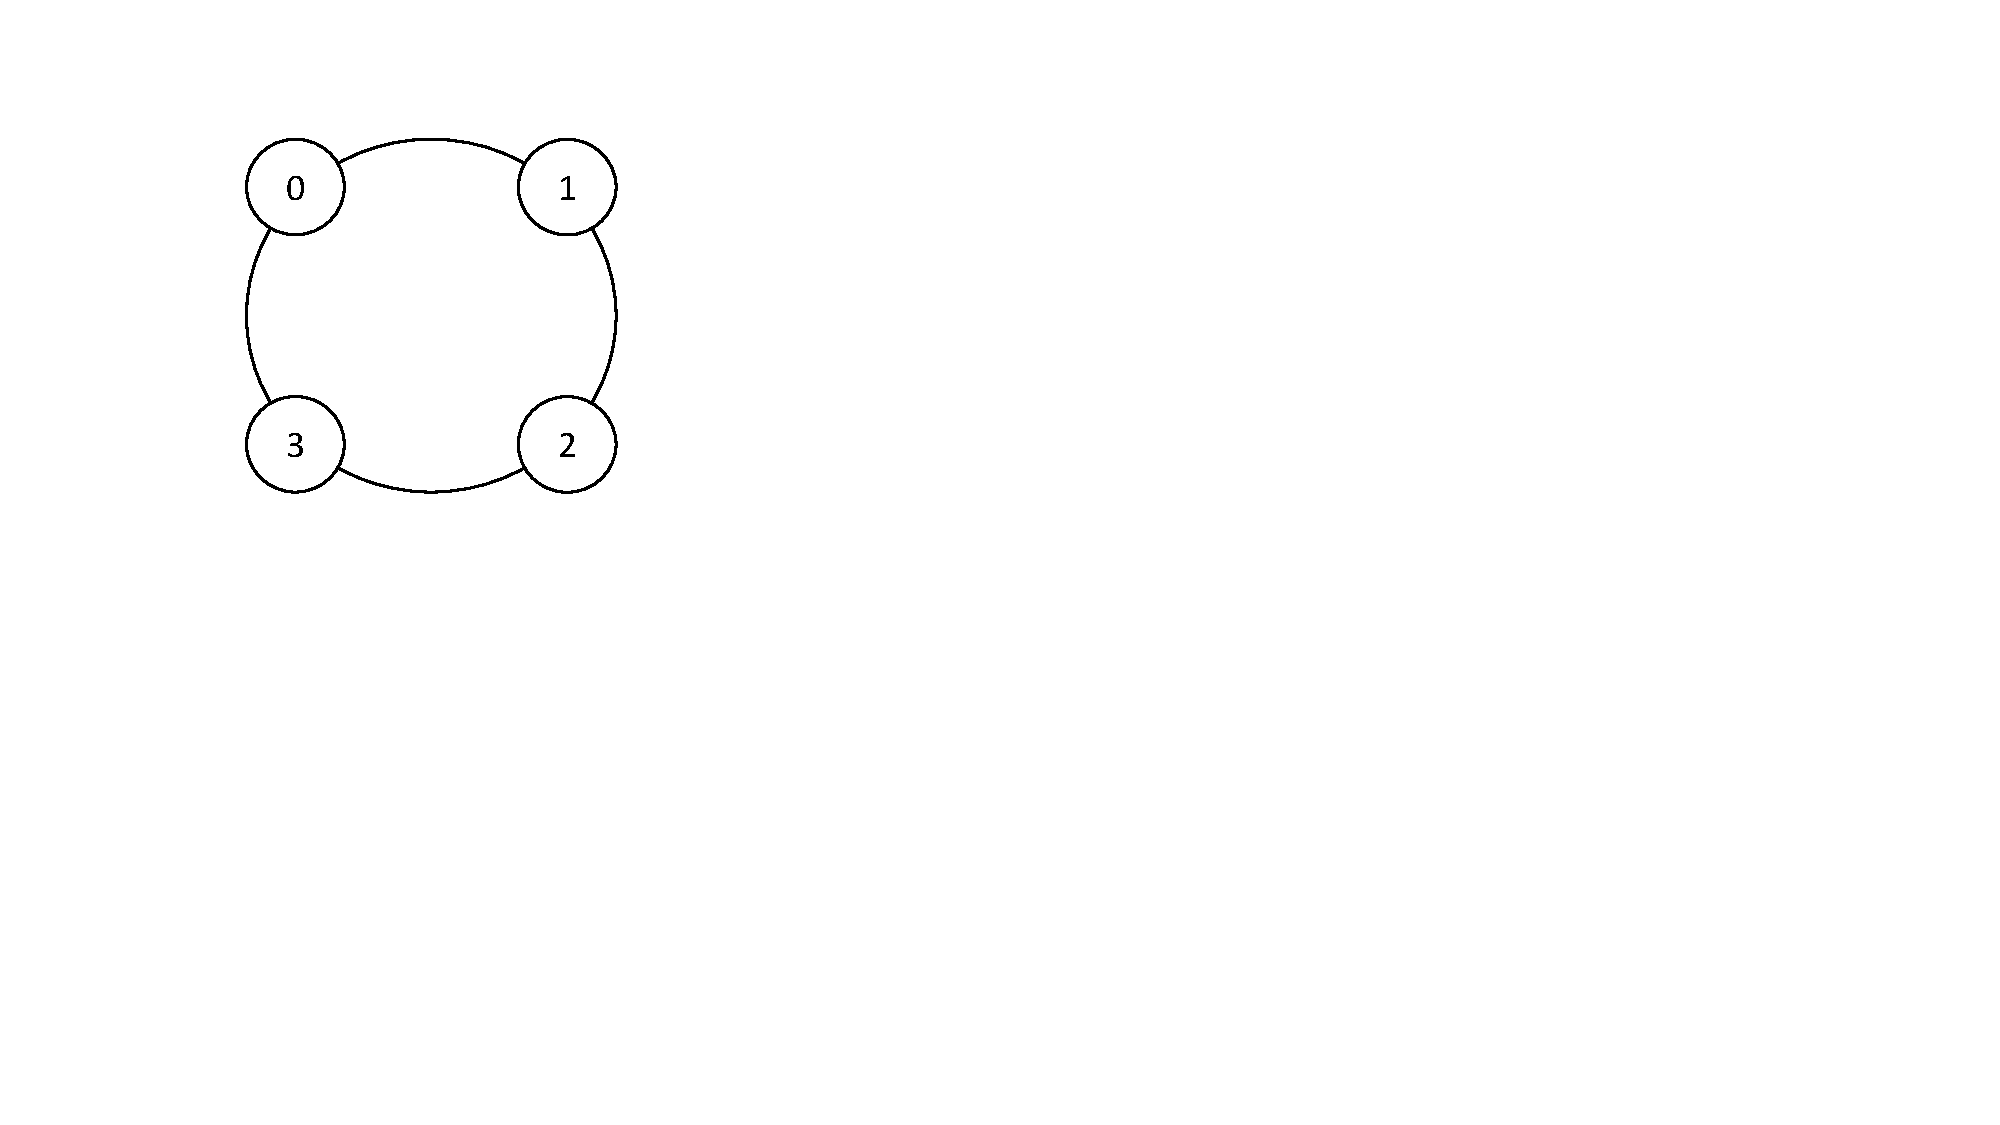
\includegraphics[scale=1.0]{Example-Bubbles}
\end{center}
\end{frame}
%
\begin{frame}
{Illustrative Example}
\[ \mu = \left (\begin{array}{c}
\mathbb{E}[x_0] \\
\mathbb{E}[x_1] \\
\mathbb{E}[x_2] \\
\mathbb{E}[x_3]
\end{array}  \right) = \left (\begin{array}{c}
0 \\
0\\
0 \\
0
\end{array}  \right), \Sigma =  \sigma^{2} \left( \begin{array}{cccc}
\rho^{0} & \rho^{1} & \rho^{2} & \rho^{0} \\
\rho^{1} & \rho^{0} & \rho^{1} & \rho^{2} \\
\rho^{2} & \rho^{1} & \rho^{0} & \rho^{1} \\
\rho^{1} & \rho^{2} & \rho^{1} & \rho^{0} \\
\end{array} \right)
\]
\\
\pause
Realization of utility for item $0$ is $y$, then updated beliefs are:
 \[ (\mu \mid x_0 = y) =\left (\begin{array}{c}
\rho y  \vspace{0.15cm} \\
\rho^{2} y  \vspace{0.15cm} \\
 \rho y \\
\end{array} \right), (\Sigma \mid x_0 = y) =  \left( \begin{array}{ccc}
\frac{3}{4} & \frac{3}{8} & 0 \vspace{0.15cm} \\
\frac{3}{8} & \frac{15}{16} & \frac{3}{8} \vspace{0.15cm}  \\
0 &\frac{3}{8} & \frac{3}{4}  \\
\end{array} \right)
\]
\begin{enumerate}
\item If $y > 0$, then always consumes item 1 or 3
\item If $y < 0$, then consumes item 2 unless sufficiently risk-averse
\end{enumerate}
\end{frame}
%
\begin{frame}
{Filter Bubble Effects}
\begin{center}
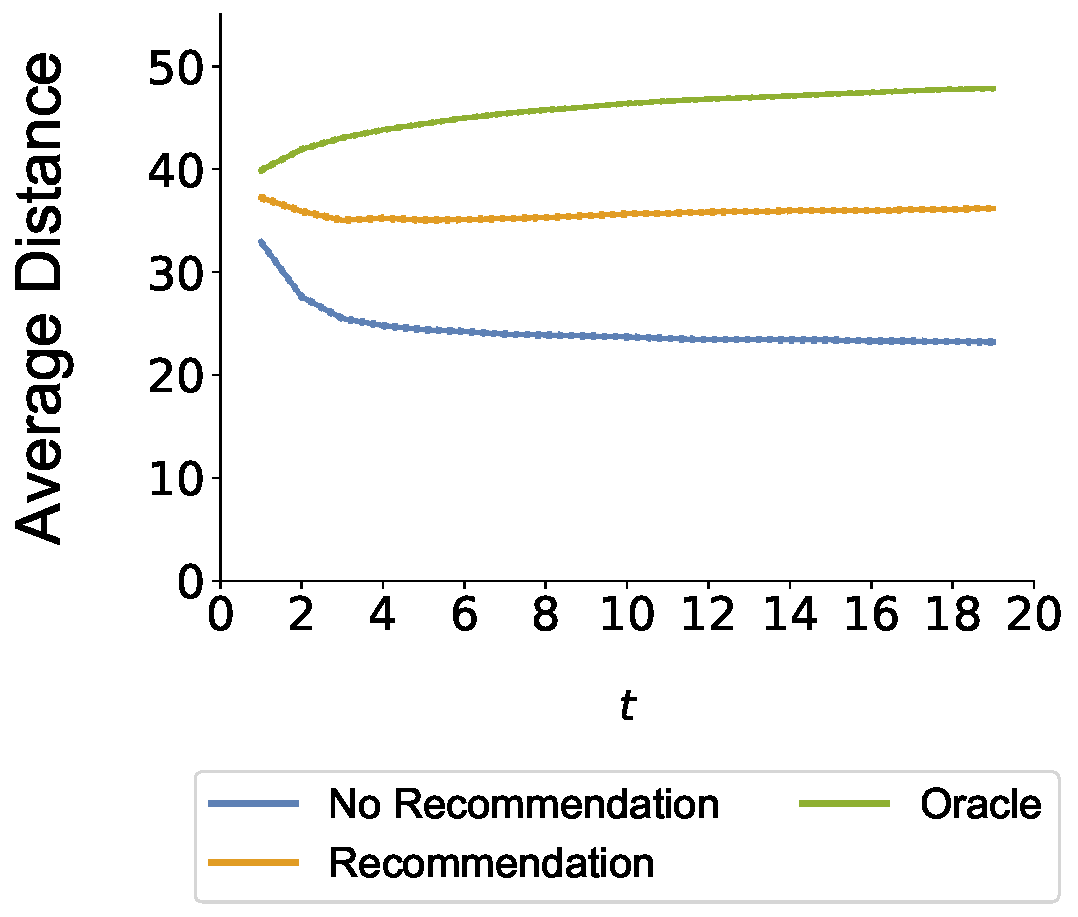
\includegraphics[scale=0.5]{rho_pos_consumption_dist_N_200T_20_overall}
\end{center}
\end{frame}
%
\begin{frame}
{Informational Spillovers Lead to Filter Bubble Effects}
\begin{center}
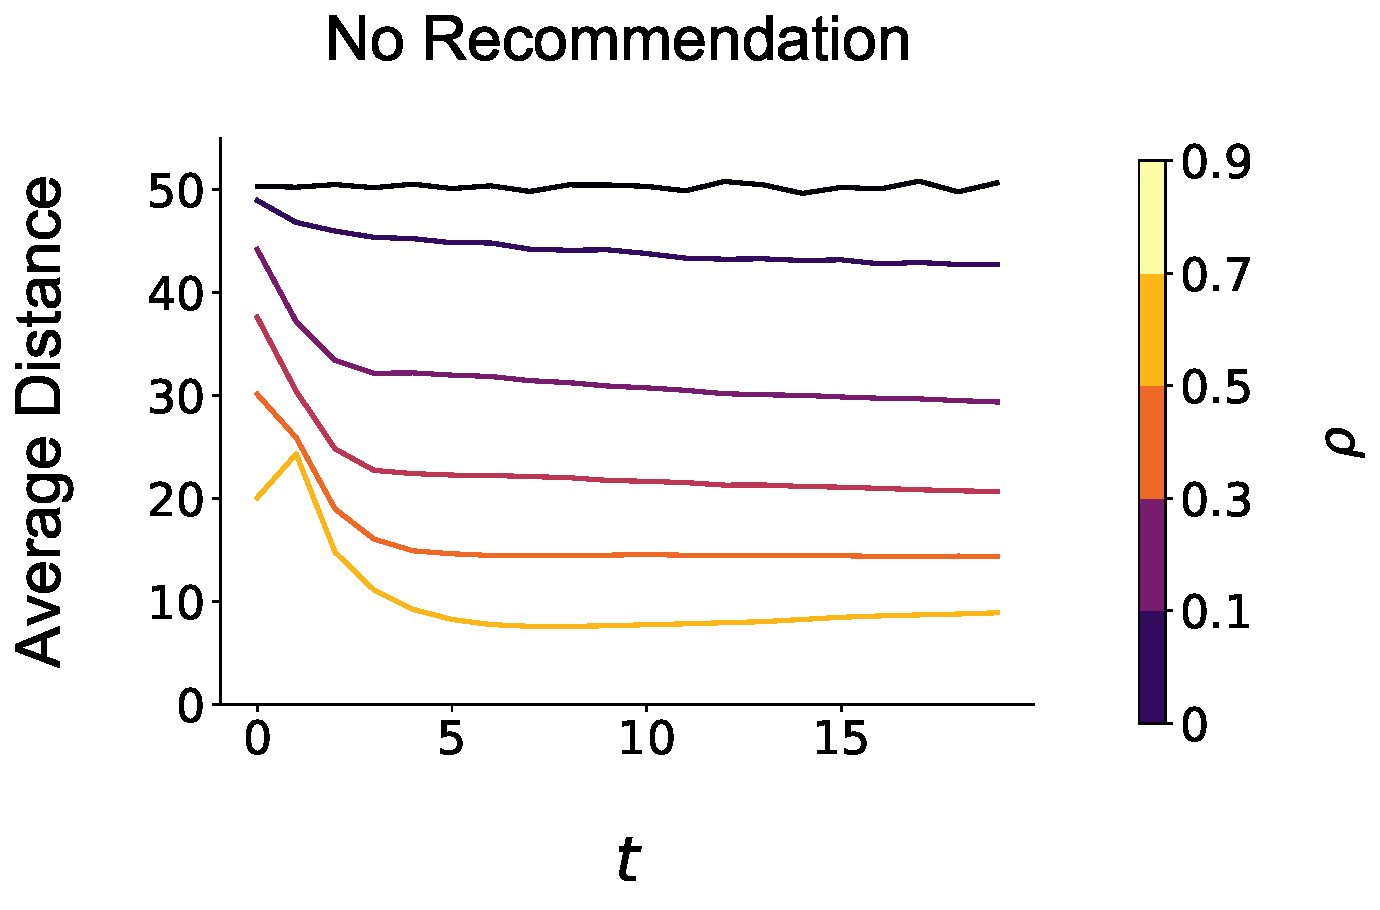
\includegraphics[scale=0.5]{rho_consumption_dist_N_200T_20}
\end{center}
\end{frame}
%
\begin{frame}
{Additional Results}
\begin{enumerate}
\item \textbf{Filter bubble effects amplified by risk aversion}
    \begin{enumerate}
    \item Spillover reduces uncertainty
    \end{enumerate}
\item \textbf{RS increases homogeneity}
    \begin{enumerate}
    \item Coordination around high common value component items
    \end{enumerate}
\item \textbf{Diversity vs. Welfare}
    \begin{enumerate}
    \item Without RS, diversity and welfare negatively correlated
    \item With RS, diversity and welfare uncorrelated
    \end{enumerate}
\item \textbf{Welfare Gains from RS}
\begin{enumerate}
\item Decreases as correlation between valuations increases
\end{enumerate}
\end{enumerate}
\end{frame}
%
\begin{frame}{Towards Recommendation System Design}
\begin{enumerate}
\item \textbf{Folk wisdom}: accurate recommendations not necessarily the most useful
\pause
\item Suppose user liked \textit{John Wick}; recommend \textit{John Wick: Chapter Two}?
\pause
\item Recommender systems traditionally ignore inference users themselves make and ignore user beliefs entirely
\pause
\item \textbf{Our approach}:
    \begin{enumerate}
    \item Goal: pairing prediction with valuable information
    \item Valuable information: steering user behavior towards better choices %via new information
    \item Implications: Collect data not only on post-consumption ratings but also on pre-consumption \textit{beliefs}
    \end{enumerate}
\end{enumerate}
\end{frame}
\end{document}
